\scanpage{134}
\mspage{66}
termes, il faut introduire, \deleted{\unsure{des cas}}
pour un morphisme
\diagram{\( (218) \)\qquad\begin{tikzcd}[ampersand replacement=\&]
\Delta_r\arrow[r,no head,"\alpha"]\&\Delta_{r'}
\end{tikzcd}},
un \uline{morphisme correspondant} de groupoïdes
\diagram{\( (219) \)\qquad\fbox{\begin{tikzcd}[ampersand replacement=\&]
\widetilde\Pi_{\Delta_{r'}}\arrow[r,"\widetilde\alpha^*"]\&\Pi_{\Delta_r}
\end{tikzcd}}}
qu'on appellera l'\uline{hom de générisation}
\margin{\figure{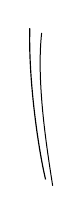
\begin{tikzpicture}[x=1cm,y=1cm]
\draw[line width=.42pt] (0,2) .. controls (-.02,1.38) and (.10,.50) .. (.20,.08);
\draw[line width=.36pt] (.15,1.94) .. controls (.08,1.31) and (.22,.45) .. (.29,0);
\end{tikzpicture}}}
associé à $\alpha$. Comme $\alpha$ se factorise
canoniquement en un hom surjectif
suivi d'un hom injectif de simplexes,
on est ramené à examiner séparément
les deux cas. Mais si $\alpha$ est surjectif
(``hom de dégénérescence''), \deleted{l'homomorphisme}
\inserted{on a $\alpha(0)=0$}
donc on est dans le cas déjà envisagé --
\deleted{\unsure{correspondant}}\inserted{d'ailleurs} dans ce cas
\diagram{\begin{tikzcd}[ampersand replacement=\&]
D^*_{\Delta_{r'}}\arrow[r]\&D^*_{\Delta_r}
\end{tikzcd}}
\unsure{se}
décompose en des morphismes \unsure{:|;}
\diagram{\( (220) \)\qquad\begin{tikzcd}[ampersand replacement=\&]
D^*_{d'_0,-\,-,d'_{r'}}\arrow[r]\&D^*_{\unsure{d_0^{\deleted{\prime}}|d'_0},-\,-,\unsure{d_r^{\deleted{\prime}}|d'_r}}
\end{tikzcd}},
$(d_0,-\,-,d_r)$ est déduite de $(d'_0,-,d'_r)$
en \unsure{réécrivant} cette suite, en répétant certains
de ses éléments -- et \deleted{les} alors (220) est
un iso -- donc \uline{si $\alpha$ est un hom}
\margin{On voit que la
considération des
$\widetilde\Pi_{d_0-d_r}$, $\Pi_{d_0,-d_r}$
pour $d_0,-\,-,d_r$ non
\uline{strictement} \unsure{décroissants|décroiss.}, et
celle de $\alpha^*$, pour $\alpha$ \unsure{non}
\uline{stricts} \unsure{croissants|croiss.}, est de
la poudre aux yeux
simplement !}
\margin{133}
